\chapter{Synthesis}
\label{synthesis}
\newpage

\noindent

\section{Summary}

This thesis can be summarized in one sentence:
we've developed the tools to measure the
error we make in phylogenetic inference and
applied it on one non-standard speciation model.
Within this chapter, I will put this into perspective.
I will first take a look at the most basic thing produced,
which is the software underlying the research,
as this is the easiest to describe objectively. 
From this rather plain foundation, I will move on 
to the way the actual research is done and ending
with the implications for the field of biology.

\subsection{Software}

A simple way to quantify the amount of work
is to count the lines of code and compare with related
software. In figure \ref{fig:sloccount} (and table \ref{tab:repos})
I show the number of
(non-empty) lines of code for the packages I developed, the packages
I maintain, the packages I contributed to, as well as BEAST2.
BEAST2, which is the foundation of the work in this thesis, 
has the most lines of code, above 110k. After that comes
\verb;beautier; (27k lines), \verb;phangorn; (18k), 
\verb;pirouette; (17k), \verb;daisieme; (14k), 
\verb;DAISIE; (12k) and \verb;razzo; (8k). 
\verb;beautier; is an R package that creates a BEAST2 
input file, and is part of the \verb;babette; package suite, as described
in chapter 2. 
\verb;phangorn; is a general phylogenetics package of which I fixed some bugs.
\verb;pirouette; is the package described in chapter 3. 
\verb;daisieme; is part of a project that did not reach full fruition yet (see below).
\verb;DAISIE; is an R package developed in our group, with 42 citations on
Google scholar. \verb;razzo; is the package described in chapter 4.
Summing up the packages of which I wrote most of the code, results
in 90k lines of code. This number of lines is still less than 
BEAST2 (with 110k), except all written in half the time. Also note that
BEAST2 has 26 collaborators, of which 6 contributed more than 1k lines of code.

\begin{figure}[]
  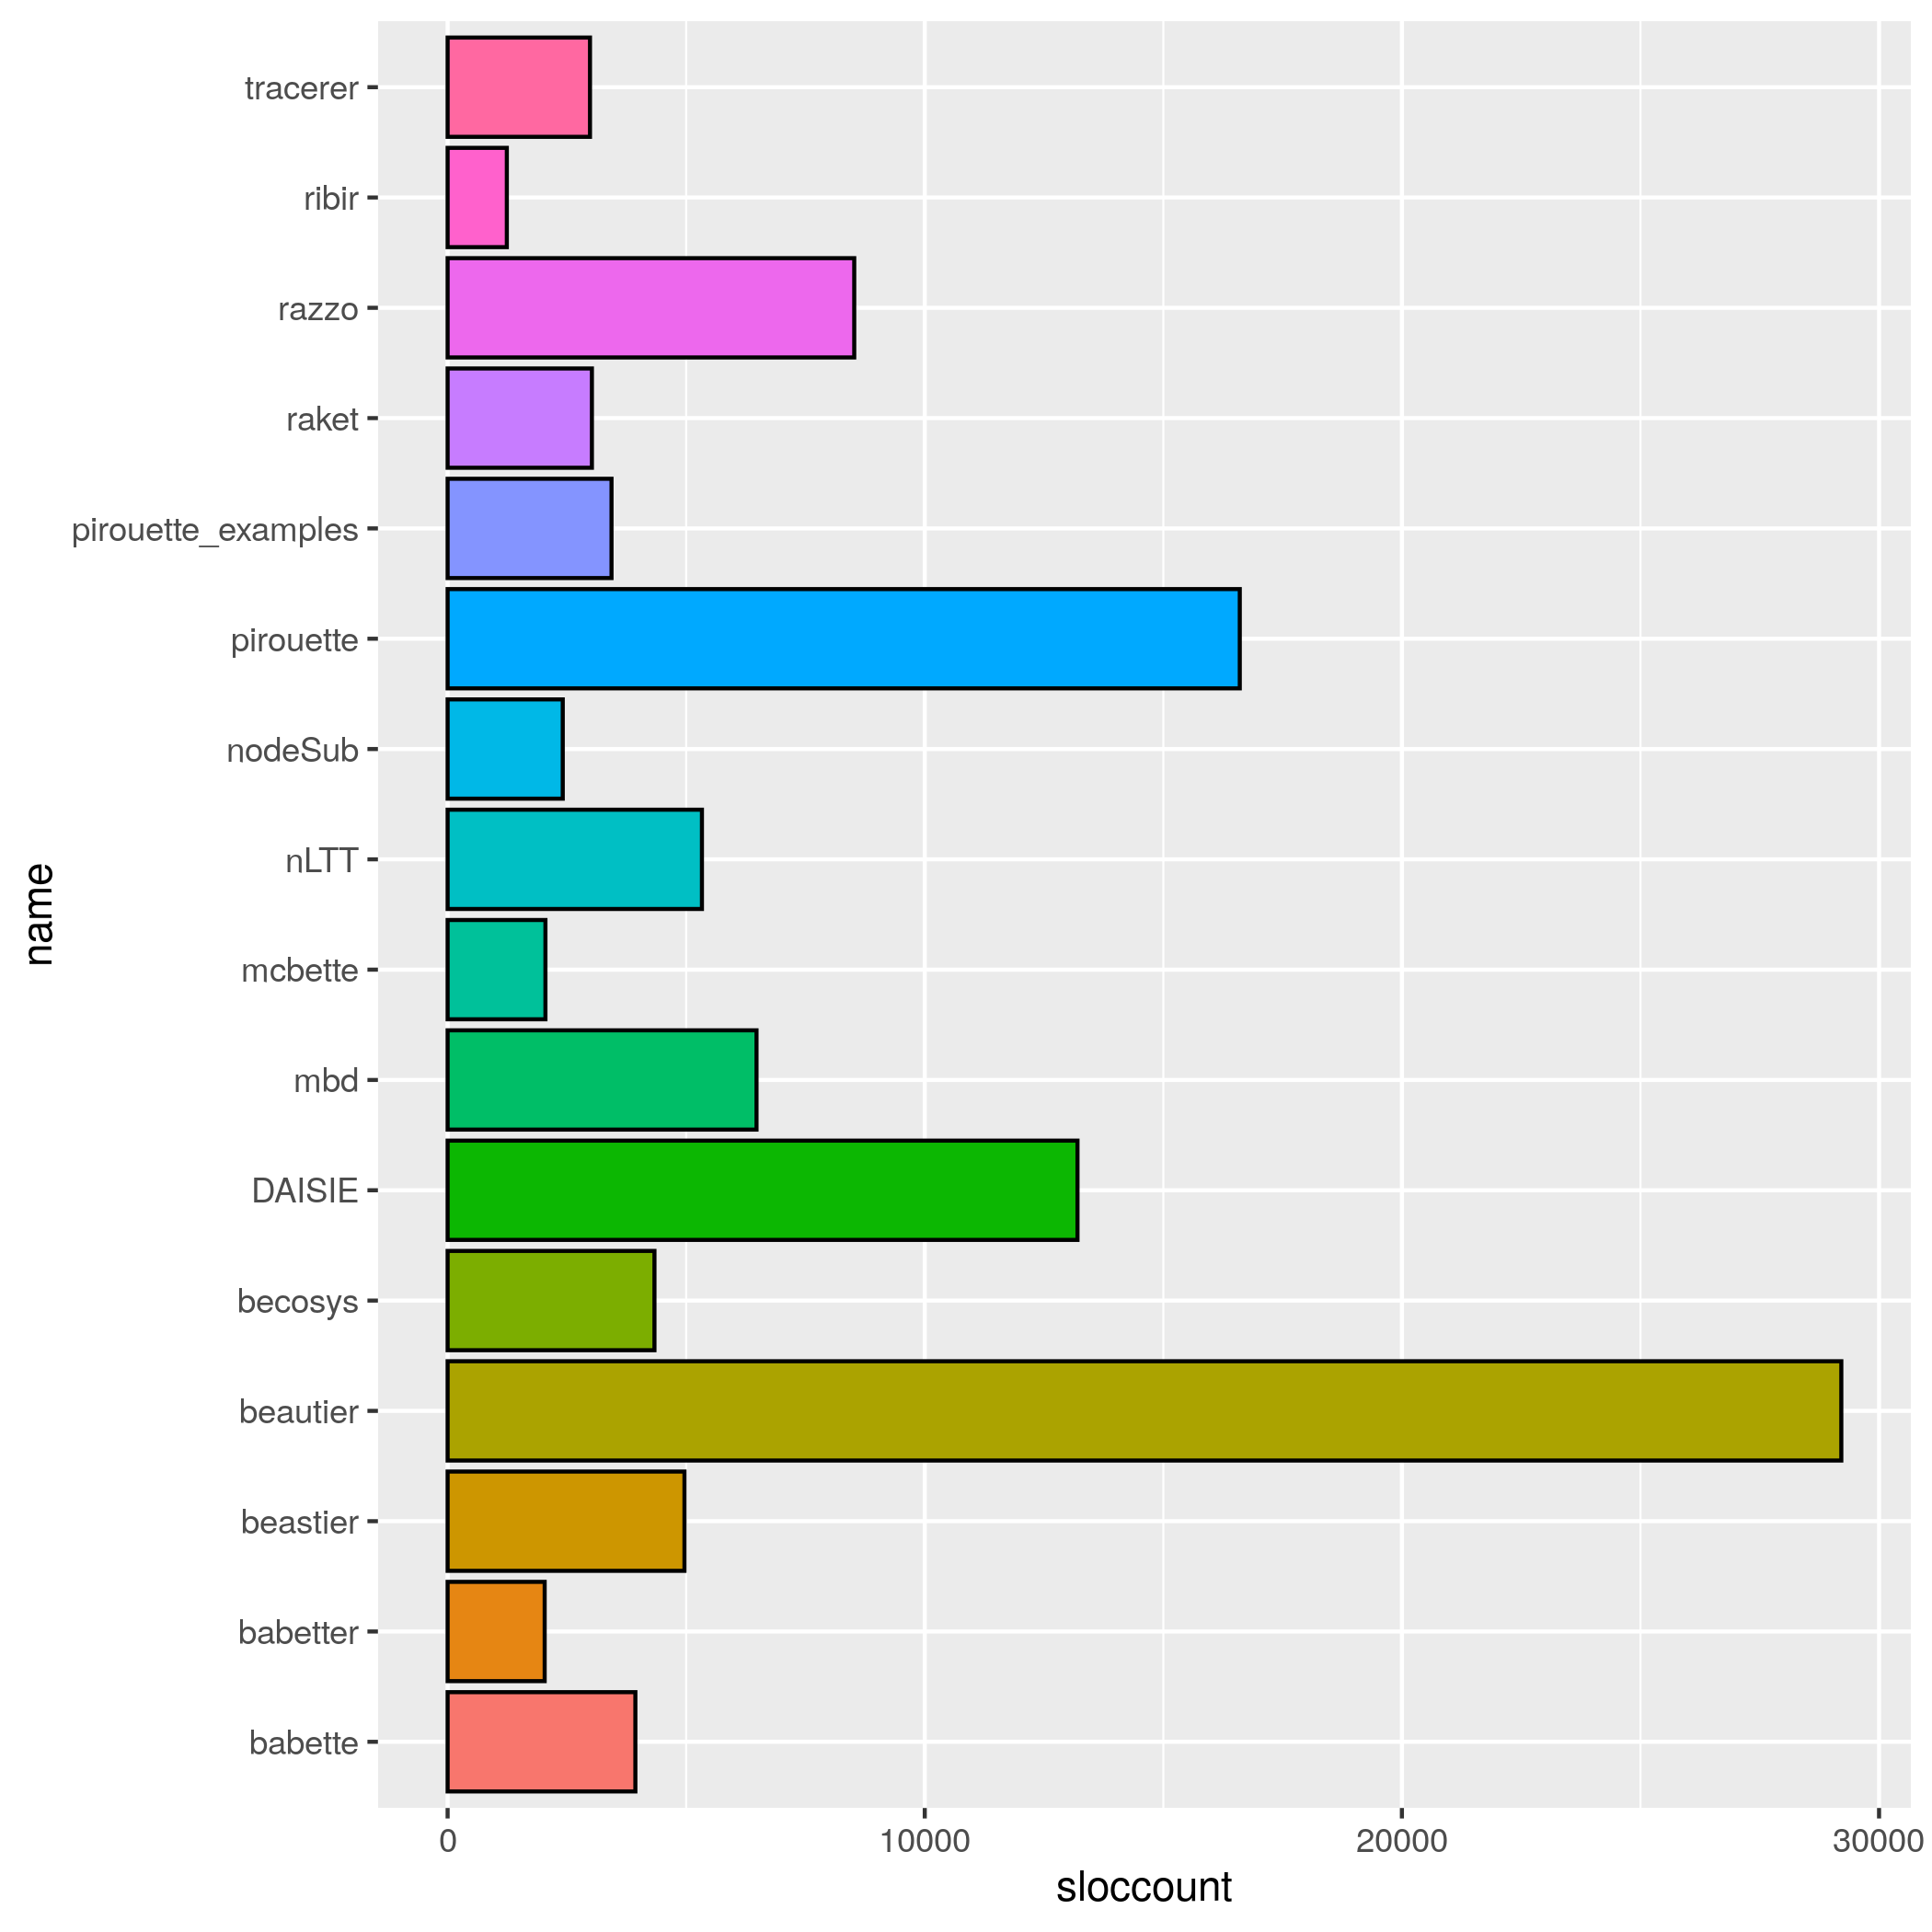
\includegraphics[width=0.8\textwidth]{sloccount.png}
  \caption{
    SLOCcount: number of (non-empty) source code lines per repository 
  }
  \label{fig:sloccount}
\end{figure}

\paragraph{Quality}

Judging code by the number lines of code is simple, but this is irrelevant 
to estimate the quality of the software.
Here I will highlight some indirect evidence of software quality,
for the software listed in figure \ref{fig:sloccount}.
To start with, all software in figure \ref{fig:sloccount} uses a
continuous integration (CI) service, which is known to significantly 
increase the number of bugs exposed (\cite{vasilescu2015}) and increases
the speed at which new features are added (\cite{vasilescu2015}).
A CI service is automatically activated when a developer puts a new version of
his/her software online. The CI service will create a virtual computer from
scratch, build the software and run it. These virtual computers can
be of multiple operating systems. 
Where BEAST2 and \verb;DAISIE; are tested on Linux only, \verb;beautier;,
\verb;pirouette; and my other R packages are tested to run under MacOS and
Windows as well, assuring users of the three major operating systems
can actually run these.

A simple metric to get an idea of code quality is the code coverage.
Code coverage correlates with code quality (\cite{horgan1994,del1995correlation}). 
The code coverage is the percentage of lines
that is actually executed by tests. 
Writing tests is fundamental for writing quality code.
These tests are usually run by the CI, each time a developer puts a new version
online. Ideally all lines of code are tested. 
As can be seen in table \ref{tab:repos}, all \verb;babette; packages
have a 100\% code coverage, compared to BEAST2, with an 
unknown/undisclosed code coverage, \verb;phangorn; with approximately
70\%, followed by \verb;DAISIE; with approximately 60\% 
\footnote{
  I used the code coverage of the 'geodynamics' branch, 
  as 'master' has 0 \%
}.

Another measure to improve code quality is peer review. Similar to
academic manuscripts, also code can be peer reviewed. 
For R code, rOpenSci is the non-profit organisation that does so.
Note that a prerequisite for a code review by rOpenSci is that code coverage is 100\%,
therefore \verb;phangorn; and \verb;DAISIE; are not yet eligible.
The five packages of the \verb;babette; package suite have been reviewed, 
where \verb;mcbette; is under review. 
The full process of the review of \verb;babette; took approximately one year,
as this is done in the free time of both me and the reviewers.
Mostly due to this, there has not been time yet to have \verb;pirouette; reviewed.

\paragraph{Relevance}

The relevance of software is another facet: one may write big pieces
of software of high quality, but if nobody uses it, the work is 
still irrelevant.

One way to estimate the relevance is to measure the number of CRAN downloads
per month. CRAN is a central repository for R packages, which keeps
track of the number of downloads. By this measure, as of March 9th 20202,
\verb;phangorn; is most relevant, with 15k downloads per month, followed 
by \verb;beautier; (975), \verb;tracerer; (849) and \verb;DAISIE; (736). Because BEAST2
is not an R package, it is absent from this list.

Another way to estimate the relevance is to measure the number of stars
given on GitHub. GitHub is a website that hosts source code
and that allows to develop software collaboratively.
Logged-in users (there are 40 million) can give a star to a project
to indicate his/her appreciation of the project.
Going through the projects in \ref{fig:sloccount}, most stars
are given, as of March 9th 2020, to BEAST2, with 134, followed
by \verb;phangorn; with 110 and \verb;babette; with 20 stars.
After \verb;beautier; (6), \verb;tracerer; (5), \verb;beastier; (5)
and \verb;mcbette; (4), \verb;pirouette;, \verb;DAISIE; and \verb;nLTT; have 3 stars.
For repositories with 3 or less stars, these stars are given by
the developers themselves and thus less relevant to indicate
the relevance of a project.

\paragraph{Community}

A time-consuming aspects of developing software is taking care of its
users, which includes the developer(s).

Users expect that R packages are easy to install.
The R community has a centralized website from which packages
can be installed easily, called CRAN (short for 'Comprehensive R Archive 
Network').
Therefore, a developer aims to get his/her package on CRAN.
There are, however, many 
guidelines (see \url{https://cran.r-project.org/web/packages/policies.html}) before 
a package gets accepted on CRAN.
These guidelines exist to guarantee a minimum level of quality.

The most important guideline when submitting an R package to CRAN,
is that all its dependencies are on CRAN. Figure \ref{fig:dependencies}
shows the dependencies of the R packages used in this thesis, showing that
three out of the five \verb;babette; packages depend on the two others. 
It would take one full year to get all packages on CRAN.

\begin{figure}[]
  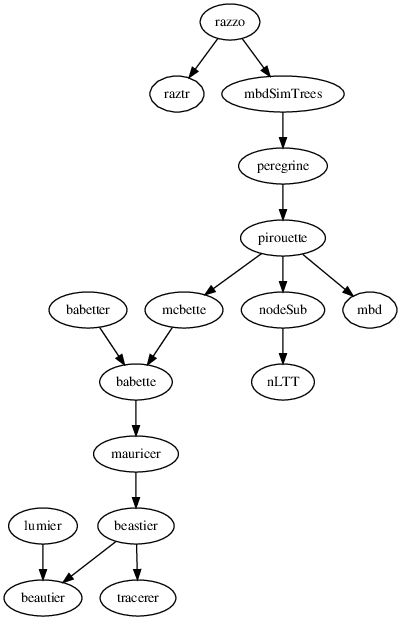
\includegraphics[width=0.6\textwidth]{dependencies.png}
  \caption{
    Minimal spanning tree of the dependencies of the R packages used in this
    thesis. Arrows go from a package (at the tail), 
    to the package it depends on (at the head). For example,
    'beastier' depends on 'beautier'. The packages on CRAN are 'beautier',
    'tracerer', 'beastier', 'mauricer' and 'babette'.
  }
  \label{fig:dependencies}
\end{figure}

A consequence of taking care for the user, is that there should be
a version of each of the packages that always works, regardless of ongoing
development. If a top-level package, say \verb;razzo; requires some different 
functionality of a bottom-level package such as \verb;beautier;, there
can be a cascade of new versions: a change in \verb;beautier; 
can cause a change in any of the packages that depend on its.
Due to this, \verb;beautier; (as of 2020-03-10) is at its fourth CRAN version.

Users expect that the code they use has a certain quality,
as they will depend on it. There are multiple ways to verify
code quality. A popular feature is the use of status badges: 
dynamic images shown in the README of a project that 
signal a certain aspect of it, such as build status and code coverage.
Additionally, code should be open, so the style and extent of tests can
be verified. An example of a package that can improve in this
regard is the \verb;ape; package (\cite{ape}), which contains
a class for a phylogeny. It is possible to read the R code \verb;ape; consists
of from a CRAN submission. Except for that, there is no way to 
verify the code quality and development process: code is added by sending 
it per email, there is no website (such as
GitHub) that tracks the development of the code and the tests are 
unavailable (although they apparently exist, according to personal 
communication with the maintainer of the package, Emmanuel Paradis). 

Users also need documentation to learn to use a new package.
One piece of documentation is an academic paper describing the functionality
of a package. Such a paper is useful for getting the idea behind a package.
User group meetings and tutorials (articles and videos) are better for
learning how to use a package. BEAST2 has a user group meeting every half year,
as well as dozens of tutorials (three of which I wrote). Specific to
the R programming language is the vignette, a kind of documentation that
can run a package's code. Counting the vignettes, \verb;beautier; has four, 
\verb;phangorn; has two, \verb;pirouette; has six, \verb;daisieme; has 
one (but well, it is unfinished), \verb;DAISIE; has two and \verb;razzo; has two. 
The complete \verb;babette; package suite has
22 vignettes.
Additionally, for \verb;babette;, and \verb;pirouette; there are nine 
video's to be downloaded or to be streamed from YouTube.

Users also expect a community: a place where they can ask questions,
submit bug reports and contribute new code. GitHub has a checklist of
seven recommended community standards (see, for 
example, \url{https://github.com/ropensci/babette/community}): having 
a one-line project description, 
having a README file, having a Code of Conduct, having a
document that describes how to contribute, having specified a software license, 
as well as having template texts for Issues (among others, bug reports
and feature request) and pull request (which is a code contribution of any type).
Of these seven standards, BEAST2 has three, 
\verb;beautier; all, \verb;phangorn; has two, \verb;pirouette; and \verb;daisieme; have all,
\verb;DAISIE; has two and \verb;razzo; has six.

\subsection{Scientific method}

Now that we have an idea of the amount of practical work underlying
this thesis, let's take a look at the scientific methods used.

\paragraph{Reproduction in practice}

Reproducibility is an essential ingredient of science (\cite{mcnutt2014reproducibility}).
The inability to reproduce experiments resulted in the so-called 'reproducibility
crisis', which still is ongoing (\cite{schooler2014metascience}).

There are multiple threats to deliver reproducible 
science (\cite{munafo2017manifesto}).
The two threats most relevant in the context
of my research are HARKing and p-hacking (see 
figure \ref{fig:manifesto} for all threats).
HARKing, short for 'Hypothesis After Results are Known' is the practice
to write down a hypothesis after having done an experiment.
p-value hacking is the process of changing the analysis up until
something significant is found. 

\begin{figure}[]
  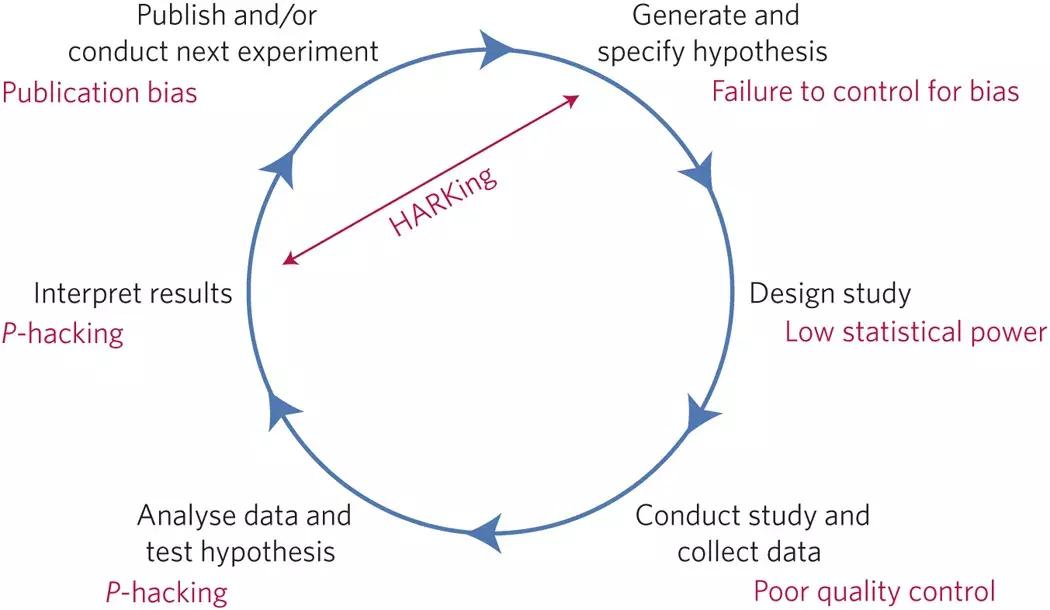
\includegraphics[width=0.8\textwidth]{munafo2017manifesto_fig_1.jpg}
  \caption{
    Threats to reproducible science, from \cite{munafo2017manifesto}
  }
  \label{fig:manifesto}
\end{figure}

The drawback of HARKing and p-hacking is that it leads to
irreproducible science. From HARKing, hypotheses that were not under
investigation, suddenly get some credibility, obtained from a
random/no effect. p-value hacking gives more credibility 
to an experimental variable having an effect than warranted.
It is estimated that 85\% of the publications in biomedical sciences
is a waste of resources (\cite{chalmers2009avoidable}) (but note
that this estimation is based on a logic reasoning, instead
of empirical data), although the situation has improved 
since \citet{macleod2014biomedical}. 

\paragraph{Assuring reproduction in practice}

One way to protect one's research from HARKing and p-hacking
is the use of preregistration. Preregistration is the act of
publishing an experiment's hypothesis, methods and analysis,
before the experiment is finished. 

\paragraph{Reproduction in this thesis}

The work in this thesis adheres to many of the best 
practices for reproducible research (\cite{munafo2017manifesto}).
All papers in this thesis are Open Access.
The \verb;razzo; experiment was not pre-registered, as a lighter variant was used:
code, manuscript and communication went via GitHub. GitHub is a website that
allows people to collaborate. A feature of GitHub is that it keeps track
of all changes. For \verb;razzo;, the hypotheses and methods were written
before the first results, and it is possible to verify this.
Also the pilot runs of \verb;razzo; can be found, as well as their results.
By being completely open, we protected ourselves against HARKing and
p-hacking.

\paragraph{Open Science}

Where reproducible research is an important facet of the scientific method,
there is the Open Science movement that goes further: not only
should there be openness in the research conducted,
also the scientific article, resulting data, and software should be open.
In that way, the scientific knowledge is accessible to all (among other,
the tax payer) and can be reproduced by all. 

All the academic articles have been put on bioRxiv before publication.
bioRxiv is a pre-print server, meaning that it stores academic manuscripts
before these appear in print. Although the manuscript may not have been
peer-reviewed, it is allowed to upload the version after peer-review,
without the journal-specific layout. In that way, anyone can download
my academic articles. Additionally, the GitHub repository that hosts
the article is also accessible.

All the academic articles I published are Open Access. 
In this way, anyone can download them without any paywall.

All the academic articles are created by free and open source software ('FOSS').
Which means that anyone, regardless of operating system, can
read these without any financial cost.

All the experiments are performed with FOSS only.
Which means that anyone, regardless of operating system, can
reproduce these, without any financial cost.

\subsection{Biology}

Now that we have an idea of practical work and scientific methods underlying
this thesis, we can take a look what this thesis has contributed to
increase our biological knowledge. 

\paragraph{'babette'}

Because \verb;babette; calls BEAST2, it is tempting to say that \verb;babette;
is just as relevant to the field of biology as BEAST2. 
This claim would be false, as not all aspects of BEAST2 are available
within \verb;babette;. The contribution of \verb;babette; to the field of biology, 
is that it leads to more reproducible research: where it takes multiple
programs to create, start and analyse a BEAST2 experiment, \verb;babette;
can do this from one R script. 

\paragraph{'pirouette'} 

The contribution of \verb;pirouette; to the field of biology, 
is that it gives a thoroughly-tested framework to answer
basic phylogenetic questions. The supplementary materials 
of \verb;pirouette; shows plenty of examples that can evolve into
a full academic paper when investigated more systematically.

Interestingly \verb;pirouette; can also be used to 
investigate different models of how an alignment is simulated
from a phylogeny, even though pirouette was not originally designed to do so. This was a fortunate example of the flexibility of 
\verb;pirouette; and begs the question what \verb;pirouette; will be most used for in the future.

\paragraph{'razzo'} 

The contribution of \verb;razzo; to the field of biology
is the introduction of a new tree model, 
and measuring the error we make in our phylogenetic inference when
nature follows a non-standard speciation model.
This non-standard speciation model is the multiple-birth death (MBD) tree model,
which is the first tree model that allows multiple speciation events to occur 
at exactly the same time.
The predictions of \verb;razzo; have always been straightforward:
the stronger a tree violates the assumptions of a standard tree
prior, the bigger the inference error made by that prior.
What is unknown, is the extent to which this happens.

There are some assumptions that \verb;razzo; makes that can be discussed,
which are the assumptions of the MBD tree model and the assumptions
made by the experimental setup.
Where the MBD model assumes speciation events can co-occur at exactly
the same time, one could easily argue that two speciation events
at different locations cannot happen at \emph{exactly} the same time.
The elegance of the MBD model is in the low number of parameters it
needs to generate trees in which speciation can co-occur.

The biological relevance of this project hinges on multiple unknown
facets. We did not investigate how common the MBD model is in nature,
instead the model is loosely based on one example, which is the 
adaptive radiation in Lake Tanganyika. However,
in the cases that MBD has a good fit with the data, 
the \verb;razzo; experiment can show us the error we make in our phylogenetic 
inference. From this, we may either rest assured that our inference is good 
enough, or that we really need to add MBD to the set of standard models.

\rampal{
  I have not read the razzo ms yet, but I think that you should say 
  a bit more about how relevant the model is. In the razzo ms you 
  should review the literature on the species pump which is the idea 
  underlying MBD and empirical support for it. Then you can refer back 
  to it here.
}
 

\subsection{Cancelled projects}

During my thesis, I worked on some other projects that did not make
it into this booklet. I will discuss these here.

\paragraph{'raket'} 

\verb;raket; is the ancestor of all chapters in this thesis.
It would do the same thing as \verb;razzo;, but for a different non-standard 
speciation model. This non-standard speciation model is
called the Protracted Birth-Death model (PBD), in which speciation
takes time: after a speciation event, one of the two new species is not
directly recognized as such. Up until these are recognized, the number
of species that are present (when looking back from the future) 
is underestimated.

The \verb;raket; experiment would have one extra step compared to the \verb;razzo;
experiment: in the \verb;raket; experiment, an \emph{incipient} species tree
would be simulated first, after which a species tree would be created
from it. The way to do so, is by picking incipient species to represent
a species.

One novel finding of the \verb;raket; experiment, is that the sampling
method to create a species tree is in some cases counterintuitive.
The sampling method selects which incipient species 
will represent a (good) species. For example, one can select the
incipient species that speciated most recently to represent its
species. One would expect that sampling by this method would
always result in a phylogeny that has the shortest branch lengths.
This assumption is false, however, if there is a certain type of
paraphyly, as shown in figure \ref{fig:pbd_sampling}. 
As I was interested in obtaining phylogenies with the
shortest branch lengths, the sampling method to obtain 
these was added. A similar story holds for sampling the oldest 
incipient species, which does not always result in a phylogeny with
longest branches. Dueo to this, 
from the three existing sampling methods, 
two new methods have been added.

\begin{figure}[]
  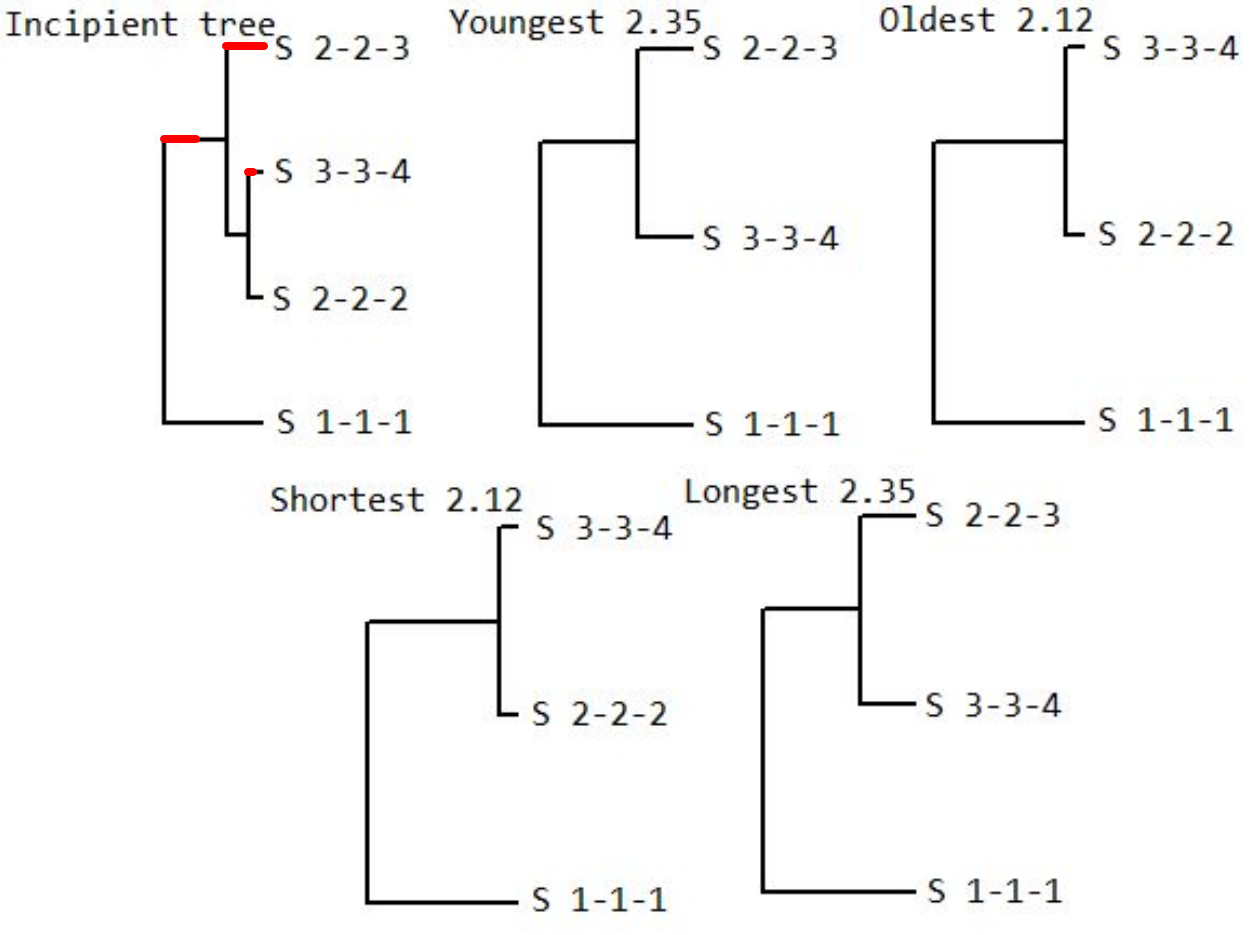
\includegraphics[width=0.8\textwidth]{raket_sampling_methods_modified.png}
  \caption{
    Sampling of PBD trees. At the top-left is an incipient species
    trees, that shows four different incipient species. Species
    'S2-2-2' and 'S2-2-3' are two different species, yet not recognized
    as such. The red edges denote a species still being an incipient
    species. The other four phylogenies are the result of four sampling
    methods. The sampling methods is shown above each phylogeny,
    as well as the sum of the branch lengths.
  }
  \label{fig:pbd_sampling}
\end{figure}

\verb;raket; would be another illustration of the inference error we make
if nature follows a non-standard speciation model. The same remarks as
\verb;razzo; apply here as well: it is unknown how well nature fits the PBD model.
In the cases that nature fits the PBD model well, then \verb;raket; would have
been able to show the extent of the inference error.

\paragraph{'daisieme'}

\verb;daisieme; (pronounce 'day-sham', similar to the French 'deuxième') is
a project based on \verb;DAISIE; (\cite{daisie}). \verb;DAISIE; is an island model,
which allows to estimate speciation, extinction and migration rates 
from one or more phylogenies. Island models, such as \verb;DAISIE;, typically
assume that the species on the mainland are fixed. \verb;daisieme; would
investigate this assumption, by simulating phylogenies that do have
mainland extinctions, estimating DAISIE parameters and comparing these 
parameters and predictions based on these parameters (such as the 
number of species and the number of colonizations) to the true parameter 
values and the true dynamics (of e.g. number of species and number of 
colonizations).

One of the predictions of \verb;daisieme; is that the immigration rate
will be overestimated when mainland extinction takes place, that is, species
colonize an island earlier than actually true. 
This prediction is caused by the estimated colonization time 
of species that we do not know the actual colonization time of.
For such a species, the colonization time is estimated with help
from (part of) the DNA sequences taken from all extant species.
For the island species of unknown immigration time, the closest mainland
relative is chosen. Of these two species, the time of their speciation
event is estimated. This time is used as the earliest time a colonization
event could have taken place, which is the best estimate possible
given the amount of information available. 
In figure \ref{fig:daisieme_example} this is depicted as the vertical
dashed line at the right. However, when the direct
mainland ancestor has gone extinct, the \emph{ancestor} of the extinct
mainland species will be compared to the island species, resulting in
an earlier estimated colonization time. 
In figure \ref{fig:daisieme_example} this is depicted as the vertical
dashed line at the left.
If colonization times are estimated to happen earlier, 
migration rate should go up.

\begin{figure}[]
  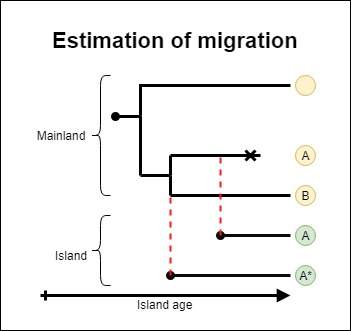
\includegraphics[width=0.8\textwidth]{daisieme_overestimation_example.jpg}
  \caption{
    daisieme example where we expect an overestimation in the migration rate.
    The top half shows the phylogeny of the mainland, which has tree
    species: A, B and an unlabelled one. The cross at the end of the
    yellow/mainland species A denotes its extinction. The vertical dashed
    red light directly left of it denotes the colonization of species A
    of the island, resulting in the green/island species A. The green/insland
    species A*, however, depicts the estimated colonization time,
    which is at the moment that mainland species A and B are formed.
  }
  \label{fig:daisieme_example}
\end{figure}

\verb;daisieme; shows the extent of the inference error we make,
for varying levels of mainland extinction. We can assume that the inference 
error increases for increasing levels of mainland extinction, but the extent
of this error will remain unknown for now. 

One preliminary result, however, is shown in figure \ref{fig:daisieme_results}.
This result points in the same way as the predictions, but a more thorough
investigation is needed before drawing conclusions.

\begin{figure}[]
  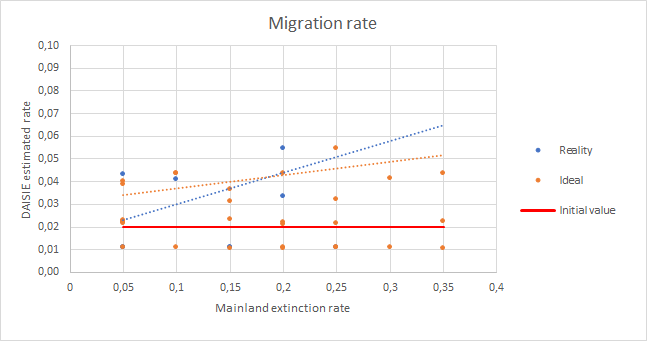
\includegraphics[width=0.8\textwidth]{daisieme_migration4.png}
  \caption{
    Preliminary daisieme result: the estimated migration rate (vertical
    axis) for different mainland extinction rates (horizontal axis).
    Orange dots show the estimated mainland extinction rates
    in an ideal situation, which is when all immigration times are known.
    Blue dots show the estimated mainland extinction rates 
    when the time of immigration needs to be estimated.
    The dotted lines show the result of a linear fit.
    The thick horizontal orange line shows the actual migration rate.
  }
  \label{fig:daisieme_results}
\end{figure}

\subsection{Reflection}

When looking back at my PhD trajectory, I see some things that I will
do again, things that I will avoid in the future, and some future work.

\paragraph{Things that I will do again} 

It was inevitable that I would write exemplary software. Writing such
software takes years, if not decades, of learning. 
Already a dozen of years before I started my PhD, I was reading the literature
regarding software development. One could argue that, would I have done 
a worse job, I would have published more academic papers. I even agree
on that! But for science as a whole, I think what I did is the superior
way to go, where the cost of the few (that is, me) benefits the many. 
For me, it always hurts when some software developer does not
care about his/her users, as I can easily envision the frustration 
this will cause.

Following the best practices for reproducible science is something
I learned during my PhD trajectory and I will definitely continue (and improve)
doing so. I think it was in my second year as a PhD student, 
when I noticed the question 'Do I believe this?' would pop up
after a scientific talk. The answer, usually, was a no. First I thought
that HARKing and p-hacking were even part of how science works
and I did not want to become such a -in my eyes: fake- scientist.
A presentation by Simine Vazire about Open Science showed me a way
to conduct science in a way that would make me believe the result,
among others to write an academic manuscript before having done
the experiment. Since then, I have taken that route. 
I am happy that if I ask myself 'Do I believe my own research findings?', 
that I can say yes.

\paragraph{Things that I will avoid} 

Already early in my PhD work, the first ideas of \verb;raket;/\verb;razzo; were
taking shape. Back then, I suggested not to pursue this line of
research, because it would be clunky and inelegant. Clunky, because
already one Bayesian phylogentic analysis takes hours. Unelegant,
because of the backbone is just a factorial design of varying
parameters. Nowadays, I still agree on this.
I think, similar to other people in phylogenetics,
that I should have pursued more light-weight and elegant experiments.

When developing a pipeline such as \verb;pirouette;, there is a tension
between (1) adding a new feature, (2) publish. The basic
and minimal pipeline is the setup without candidate models and without
twinning. Already this subset of the pipeline allows one to 
measure the inference error we make in phylogenetic inference.
The \verb;raket; paper, that was pre-registered two years ago, used only
that part of the pipeline. Instead of investigating this minimal
pipeline and publish the findings, features were added instead.
These features are the use candidate models and the addition
of a twin pipeline. 

The first extra \verb;pirouette; feature, which is the use of candidate models,
has, in my opinion, caused mostly harm to the progress in my PhD work, without adding
enough value. The main reason for this harm, is that the use of candidate
models can only run under Linux and Mac, due to a feature of BEAST2 that
only works under those two operating systems. Most desktop users, however,
use the Windows operating system, so I needed to take this into account.
Due to this, I had to write code that I would never run myself, a weird
situation. Also, my co-author Giovanni Laudanno, who uses Windows, had
a hard time to contribute to the \verb;pirouette; code. 

The second extra \verb;pirouette; feature, which is the use of a twin pipeline,
was, in my opinion, unwarranted to add before the publication of the minimal
pipeline. There is some benefit to use twinning, but I think 
it would have been superior to show this benefit by reproducing an earlier
\verb;pirouette; publication with this new feature.

\subsection{Future work}

My suggestions for future work are rather straightforward:
(1) to measure the inference error we make on \emph{standard}
speciation models, (2) to measure the inference error we make 
on \emph{other non-standard} speciation models, and (3) to
make the MBD tree model part of the set of standard models.

\paragraph{Apply 'pirouette' on standard speciation models} 

The goal of \verb;pirouette; is the measure the inference error
when a phylogeny is created by a non-standard tree model,
but a standard tree prior is used in the inference. There are,
however, only a couple of studies that investigate the
inference error when using only standard tree models.

I think it would be useful to measure the inference
error when using a standard tree model, when also
assuming that tree model in the inference. This will give the
baseline error, in a similar fashion as twinning does.
This error would be the baseline error, in a similar way that
twinning allows one to measure this. From these baseline errors,
I would enjoy to fit a mathematical model on these errors,
to be able to obtain a prediction of this error without running
the time-consuming Bayesian inference.

A next fundamental step would be to measure the inference
error when creating phylogenies using a different standard tree model
as is assumed in the inference. 
When we know the error we make when nature follows a BD model,
when assuming a Yule model, this would give a sense of scale.
It may even be that there is no reason to use BD at all,
because the inference error is too little to warrant using it!
Whatever this error, I would be curious to see how it compares
to the errors found in \verb;razzo;. 

I understand why this has not been researched: it takes too long
and there is little glory in finding this out. With \verb;pirouette;, however,
it should at least be easy to setup these experiments.

\paragraph{Apply 'pirouette' on multiple novel speciation models} 

The inference error that \verb;razzo; measures, is caused by the
mismatch of using an MBD tree, yet assuming a BD tree model.
It is easy to do this for any non-standard tree model, such as
PBD, but also a time or diversity dependent tree model. Using
different non-standard tree priors, gives us a better idea of when we can
and when we cannot use our standard tree priors.

\paragraph{Add MBD tree prior to BEAST2}

In \verb;razzo;, we measure the inference error we make, when we generate
and MBD tree and assume a BD tree model in our inference. What we
do not know is the inference error would we assume an MBD tree model in
our inference. Being able to use an MBD tree prior would give another
baseline error: the inference error when nature follows MBD and we
correctly assume this. To do so, the MBD tree prior must be added to BEAST2, 
\verb;babette; should be able to use it, then a study similar to \verb;razzo; can be done.

\references{synthesis}

\section{Supplementary materials}

In these supplementary materials, I show the raw data referred to in the main
text.

% latex table generated in R 3.6.1 by xtable 1.8-4 package
% Thu Mar 12 11:47:08 2020
\begin{table}[ht]
\centering
\begin{tabular}{p{0.2\textwidth}p{0.4\textwidth}p{0.1\textwidth}p{0.05\textwidth}p{0.05\textwidth}p{0.1\textwidth}p{0.1\textwidth}}
  \hline
name & title & sloccount & cc & ns & ndm & ndt \\ 
  \hline
aureole & R interface to the Encyclopedia of Life & 460 & 100 &   0 &  &  \\ 
  babette & Control 'BEAST2' & 3378 & 100 &  20 & 452 & 1173 \\ 
  babette\_examples & All babette examples & 149 &  &  &  &  \\ 
  babette\_examples & All babette examples & 149 &  &  &  &  \\ 
  babetter & Check babette & 1816 &  &   0 &  &  \\ 
  beast2 & BEAST2 & 111886 &  & 134 &  &  \\ 
  beastier & Call 'BEAST2' & 4757 & 100 &   5 & 709 & 4579 \\ 
  beautier & 'BEAUti' from R & 27030 & 100 &   6 & 975 & 7135 \\ 
  becosys & Unified Interface To Phylogenetics Models Of Speciation & 3989 &  78 &   0 &  &  \\ 
  DAISIE & Dynamical Assembly of Islands by Speciation, Immigration and
        Extinction & 12314 &   0 &   3 & 736 & 18000 \\ 
  daisieme & Island Diversification With Mainland Extinction & 13558 &  97 &   1 &  &  \\ 
  DDD & Diversity-Dependent Diversification & 7151 &  24 &   1 & 1951 & 70000 \\ 
  mauricer & Install 'BEAST2' Packages & 519 & 100 &   1 & 742 & 2202 \\ 
  mbd & Multiple Birth Death Diversification & 5972 &  &   1 &  &  \\ 
  mcbette & Model Comparison Using 'babette' & 2074 & 100 &   4 &  &  \\ 
  nLTT & Calculate the NLTT Statistic & 4658 &  99 &   3 & 702 & 23000 \\ 
  nodeSub & Simulate Sequences & 2055 &  53 &   1 &  &  \\ 
  PBD & Protracted Birth-Death Model of Diversification & 3437 &  57 &   1 & 649 & 28000 \\ 
  peregrine & Work With The Groninger Peregrine Computer Cluster & 1699 &  98 &   2 &  &  \\ 
  phangorn & Phylogenetic Reconstruction and Analysis & 18453 &  69 & 110 & 15000 & 420000 \\ 
  pirouette & Create a Bayesian Posterior From a Phylogeny & 16584 &  99 &   3 &  &  \\ 
  pirouette\_examples & All pirouette examples & 1596 &  &  &  &  \\ 
  pirouette\_examples & All pirouette examples & 1596 &  &  &  &  \\ 
  raket & What If Speciation Takes Time? & 2716 &  58 &   0 &  &  \\ 
  raztr & Razzo Test Results &  52 &  &   0 &  &  \\ 
  raztr & Razzo Test Results &  52 &  &   0 &  &  \\ 
  razzo & The Error if Nature is MBD & 7690 &  76 &   2 &  &  \\ 
  ribir & ribir, basic phylogenetics page & 1053 &  95 &   0 &  &  \\ 
  tracerer & Tracer from R & 2671 & 100 &   5 & 849 & 5359 \\ 
   \hline
\end{tabular}
\caption{Repository features} 
\label{tab:repos}
\end{table}


\fbox{
  \begin{minipage}{\textwidth}
  \subsection{Altmetrics}

  \itemize{
   \item 60,000 GitHub commits, 1.1k repositories, 421 stars, 242 followers
   \item 133 YouTube videos, 68 subscribers, 11k views
   \item Supervised 2 MSc students
   \item Supervised 6 BSc students
   \item Supervised 7 interns from secondary schools
   \item Organised 172 social events
   \item Since Jan 2017, presented 20 times at TECE
   \item Publish 5 packages on CRAN
   \item Passed rOpenSci peer-review for 4 R packages
   \item Taught +220 evenings about programming
  }
  \end{minipage} 
}
